\documentclass{thesis-uestc}
% \usepackage{indentfirst} 
% \setlength{\parindent}{2em} %2em代表首行缩进两个字符

\title{珊瑚-I 启动过程}{aCoral-I Boot Process}
\author{王彬浩}{Wang BinHao}
\school{信息与软件工程学院}{School of Information and Software Engineering}
\major{电子信息}{Electrical & Information}
\studentnumber{202122090410}
\version{0.1}


% require all the usepackages here
% \usepackage{algorithm2e}
\usepackage{listings}
\usepackage{xcolor}
\usepackage{fontspec}
\usepackage{caption}
\usepackage{float}


\lstset{
    basicstyle=\small, 
    breaklines,                                 % 自动将长的代码行换行排版
    extendedchars=false,                        % 解决代码跨页时,章节标题,页眉等汉字不显示的问题
    backgroundcolor=\color[rgb]{0.96,0.96,0.96},% 背景颜色
    keywordstyle=\color{blue}\bfseries,         % 关键字颜色
    identifierstyle=\color{black},              % 普通标识符颜色
    commentstyle=\color[rgb]{0,0.6,0},          % 注释颜色
    stringstyle=\color[rgb]{0.58,0,0.82},       % 字符串颜色
    showstringspaces=false,                     % 不显示字符串内的空格
    numbers=left,                               % 显示行号
    captionpos=t,                               % title在上方(在bottom即为b)
    frame=single,                               % 设置代码框形式
    rulecolor=\color[rgb]{0.8,0.8,0.8},         % 设置代码框颜色
    tabsize=4
}  




\begin{document}

\makecover

% This is a template of mutiple files.
% The folders chapters/ and misc/ have the related files

\begin{revisionhistory}
    \begin{center}
        \setlength\tabcolsep{15pt}
        \begin{tabular}{|c|p{16em}<{\centering}|c|c|}
            \hline  版本号 & 内容 & 日期 & 负责人 \\
            \hline 0.1 & 开始编写,修改latex模板,确定大纲 & 2022.05.15 & 王彬浩 \\
            \hline 1.0 & 第一版aCoral入门引导编写完成 & 2022.06.12 & 王彬浩 \\
            \hline 1.1 & 增加Ubuntu和编译器、dnw工具的下载链接 & 2022.06.14 & 王彬浩 \\
            \hline 1.2 & 修正配置环境时的操作 & 2022.06.14 & 王彬浩 \\
            \hline \Version & 修改3.1 & 2022.07.05 & 王彬浩 \\
            \hline
        \end{tabular}
    \end{center}



\end{revisionhistory}



% table of contents
\thesistableofcontents

% thesis contents
\chapter{Bootloader}


\chapter{aCoral启动}
2440上电之后,CPU将从0地址处开始取指执行指令。如果将aCoral程序存放在Norflash中,并通过mini2440开关S2选择Norflash启动,则Norflash从硬件层面上被映射为0地址开始的一段地址;
如果将aCoral放在Nandflash中,并且通过S2开关选择Nandflash启动,则开发板在上电后自动将Nandflash前4KB内容复制到开发板上的一块SRAM中。
这块SRAM我们称为Stepping Stone(垫脚石),并且Stepping Stone的地址就是从0地址开始。所以,不论选择何种启动方式,2440都将从0地址开始执行第一行代码。

图\ref{复位后S3C2440A的存储器映射}显示了复位后S3C2440A的存储器映射情况,详细请参考S3C2440中文手册第五章。
\begin{figure}[h]
	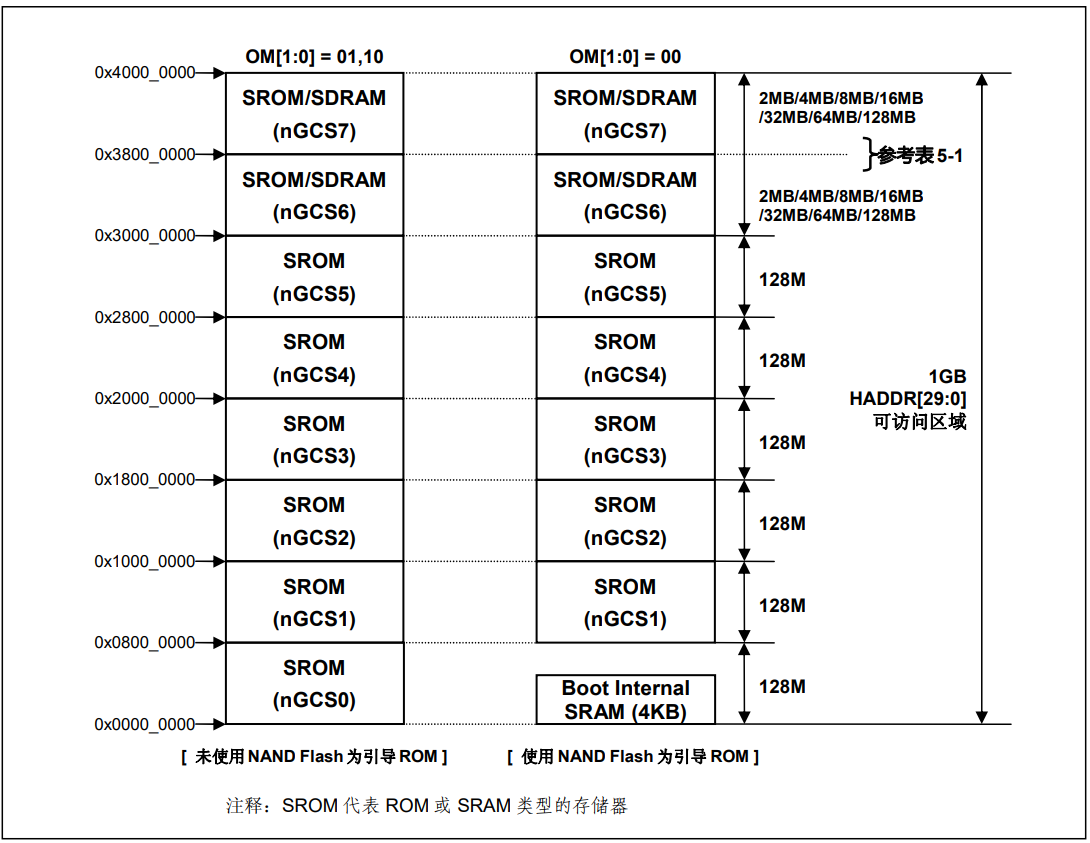
\includegraphics[width=\textwidth]{复位后S3C2440A的存储器映射.png}
	\caption{复位后S3C2440A的存储器映射}
	\label{复位后S3C2440A的存储器映射}
\end{figure}


之前说到,aCoral的bootloader其实就是
\begin{lstlisting}
 hal/s3c2440/src/start.S 
\end{lstlisting}

我们将其称为aCoral的启动文件。启动文件中,这行跳转指令就是整个aCoral的入口,将被烧录在Nandflash或Norflash的0地址。
\begin{lstlisting}
__ENTRY:
	b	ResetHandler
\end{lstlisting}

这句跳转程序将跳转到ResetHandler标号处,执行一些上电之后的硬件初始化工作,包括关闭看门狗、配置时钟、堆栈初始化、复制OS到SDRAM等。
我们一点点来看这些代码。

\section{禁用看门狗}
\begin{lstlisting}
	@ disable watch dog timer
	mov r1, #0x53000000
	mov	r2, #0x0
	str	r2, [r1]
\end{lstlisting}

\section{关中断}
\begin{lstlisting}
	@ disable all interrupts
	mov	r1, #INT_CTL_BASE
	mov	r2, #0xffffffff
	str	r2, [r1, #oINTMSK]
	ldr	r2, =0x7ff
	str	r2, [r1, #oINTSUBMSK]
\end{lstlisting}

\section{时钟初始化}
\begin{lstlisting}
	@ initialise system clocks
	mov	r1, #CLK_CTL_BASE
	mvn	r2, #0xff000000
	str	r2, [r1, #oLOCKTIME]

	mov	r1, #CLK_CTL_BASE
	mov	r2, #M_DIVN
	str	r2, [r1, #oCLKDIVN]

	mrc	p15, 0, r1, c1, c0, 0	@ read ctrl register
	orr	r1, r1, #0xc0000000	@ Asynchronous
	mcr	p15, 0, r1, c1, c0, 0	@ write ctrl register

	mov	r1, #CLK_CTL_BASE
	ldr 	r2, =vMPLLCON	        @ clock user set
	str	r2, [r1, #oMPLLCON]
\end{lstlisting}

\section{存储空间初始化}
\begin{lstlisting}
	bl	memsetup
......
	@*************************************
	@ initialise the static memory
	@ set memory control registers
	@*************************************
memsetup:
	mov	r1, #MEM_CTL_BASE
	adrl	r2, mem_cfg_val
	add	r3, r1, #52
1:	ldr	r4, [r2], #4
	str	r4, [r1], #4
	cmp	r1, r3
	bne	1b
	mov	pc, lr
......
	@************************************
	@ Data Area
	@ Memory configuration values
	@************************************
.align 4
mem_cfg_val:
	.long	vBWSCON
	.long	vBANKCON0
	.long	vBANKCON1
	.long	vBANKCON2
	.long	vBANKCON3
	.long	vBANKCON4
	.long	vBANKCON5
	.long	vBANKCON6
	.long	vBANKCON7
	.long	vREFRESH
	.long	vBANKSIZE
	.long	vMRSRB6
	.long	vMRSRB7
\end{lstlisting}


\section{栈初始化}
\begin{lstlisting}
	bl      InitStacks
......
	@************************************
	@             堆栈初始化
	@************************************

InitStacks:
	mov r2,lr
	mrs	r0,cpsr
	bic	r0,r0,#MODE_MASK
	orr	r1,r0,#UND_MODE|NOINT
	msr	cpsr_cxsf,r1		@UndefMode
	ldr	sp,=UDF_stack		@ UndefStack=0x33FF_5C00

	orr	r1,r0,#ABT_MODE|NOINT
	msr	cpsr_cxsf,r1		@AbortMode
	ldr	sp,=ABT_stack		@ AbortStack=0x33FF_6000

	orr	r1,r0,#IRQ_MODE|NOINT
	msr	cpsr_cxsf,r1		@IRQMode
	ldr	sp,=IRQ_stack		@ IRQStack=0x33FF_7000

	orr	r1,r0,#FIQ_MODE|NOINT
	msr	cpsr_cxsf,r1		@FIQMode
	ldr	sp,=FIQ_stack		@ FIQStack=0x33FF_8000

	bic	r0,r0,#MODE_MASK|NOINT
	orr	r1,r0,#SVC_MODE
	msr	cpsr_cxsf,r1		@SVCMode
	ldr	sp,=SVC_stack		@ SVCStack=0x33FF_5800

	mrs     r0,cpsr
	bic     r0,r0,#MODE_MASK
	orr     r1,r0,#SYS_MODE|NOINT
	msr     cpsr_cxsf,r1    	@ userMode
	ldr     sp,=SYS_stack

	mov	pc,r2
\end{lstlisting}

\section{自我拷贝(loader)}
\begin{lstlisting}
	adr  r0,__ENTRY
	ldr  r1,_text_start
	cmp  r0,r1
	blne copy_self  
...
copy_self:

	ldr	r1, =( (4<<28)|(2<<4)|(3<<2) )	/* address of Internal SRAM  0x4000002C*/
	mov	r0, #0		
	str	r0, [r1]


	mov	r1, #0x2c	/* address of men  0x0000002C*/
	ldr	r0, [r1]
	cmp	r0, #0
	bne	copy_from_rom
        
    ldr	r0, =(2440)
	ldr	r1, =( (4<<28)|(2<<4)|(3<<2) )
	str	r0, [r1]
	b       copy_from_nand 
\end{lstlisting}


\section{bss段清零}
\begin{lstlisting}
	ldr  r0,_bss_start
	ldr  r1,_bss_end
	bl    mem_clear
.......
	@***********************************
	@ clear memory
	@ r0: start address
	@ r1: length
	@***********************************

mem_clear:
	mov r2,#0
1:	str r2,[r0],#4
	cmp r0,r1
	blt 1b
	mov pc,lr
\end{lstlisting}

\section{跳转至下一阶段}
\begin{lstlisting}
	ldr    pc,=acoral_start	
\end{lstlisting}

代码最终将寄存器pc设置为acoral\_start的值,表示CPU将跳转到acoral\_start函数处执行。acoral\_start函数位于kernel\\include\\core.c中
	跳到C语言部分,core.c
core.c中的acoral\_start()函数如下

这部分代码中,最重要的就是acoral\_module\_init()这个函数。这个函数将初始化aCoral的各个模块,包括中断、内存、线程等嵌入式操作系统必需的模块。初始化完成后,执行acoral\_core\_cpu\_start()函数,aCoral开始运行。


\chapter{链接脚本}



\end{document}
